\subsection{CRITERIA FOR LINEAR INDEPENDENCE}

PROPOSITION 12. Let M be a projective A-module. For elements \(x_1, x_2, \ldots, x_n\) of M to be linearly dependent, it is necessary and sufficient that there exist \(\lambda \neq 0\) in A such that

\[
\lambda x _ {1} \wedge x _ {2} \wedge \dots \wedge x _ {n} = 0.\tag{22}
\]

The condition is necessary (with no hypothesis on M), for if for example \(\lambda x_{1}\) (with \(\lambda \neq 0\) ) is a linear combination of \(x_{2}, \ldots, x_{n}\) , relation (22) holds (no. 3, Proposition 5). We show that the condition is sufficient by induction on n; for n = 1, it is a trivial consequence of the definition. Suppose therefore that n \textgreater{} 1 and that condition (22) holds for some \(\lambda \neq 0\) . If

\[
\lambda x _ {2} \wedge x _ {3} \wedge \dots \wedge x _ {n} = 0,
\]

then the induction hypothesis implies that \(x_{2},\ldots,x_{n}\) are linearly dependent and hence a fortiori \(x_{1},x_{2},\ldots,x_{n}\) are. If \(\lambda x_{2}\wedge x_{3}\wedge\cdots\wedge x_{n}\neq0\) , it follows from no. 8, Corollary 3 to Theorem 1 that there exists an alternating \((n-1)\) -linear form f such that \(f(\lambda x_{2}\wedge x_{3}\wedge\cdots\wedge x_{n})=\mu\neq0\) . Since

\[
x _ {1} \wedge (\lambda x _ {2}) \wedge \dots \wedge x _ {n} = 0,
\]

it follows from no. 8, Corollary 3 to Theorem 1 that \(\mu x_{1}\) is a linear combination of \(\lambda x_{2}, x_{3}, \ldots, x_{n}\) ; hence \(x_{1}, x_{2}, \ldots, x_{n}\) are linearly dependent.

COROLLARY. Let M and N be two projective A-modules and \(f:M\to N\) an A-linear mapping. If f is injective, then \(\bigwedge(f):\bigwedge(\mathbf{M})\to\bigwedge(\mathbf{N})\) is injective.

We prove this first under the assumption that M is free; let \((e_{\lambda})_{\lambda \in L}\) be a basis of M, so that \((e_{J})_{J \in \mathfrak{F}(L)}\) (formula (18)) is a basis of \(\bigwedge(M)\) . Suppose that the kernel of \(\bigwedge(f)\) contains an element \(u = \sum_{J} \alpha_{J} e_{J} \neq 0\) . Let K be an element minimal among the finite subsets J such that \(\alpha_{J} \neq 0\) and let H be a finite subset of L disjoint from K and such that \(K \cup H\) contains all the J (finite in number) such that \(\alpha_{J} \neq 0\) ; for all \(J \neq K\) such that \(\alpha_{J} \neq 0\) , we have therefore by definition \(J \cap H \neq 0\) and consequently (no. 8, formula (20)).

\[
u \wedge e _ {\mathrm{H}} = + \alpha_ {\mathbf {K}} e _ {\mathbf {K} \cup \mathbf {H}}
\]

belongs to the two-sided ideal of \(\bigwedge (\mathbf{M})\) , the kernel of \(\bigwedge (f)\) . We write \(e_{\mathbf{K} \cup \mathbf{H}} = e_{\lambda_1} \wedge e_{\lambda_2} \wedge \dots \wedge e_{\lambda_n}\) ; then \(\alpha_{\mathbf{K}} f(e_{\lambda_1}) \wedge f(e_{\lambda_2}) \wedge \dots \wedge f(e_{\lambda_n}) = 0\) ; by virtue of Proposition 12, the elements \(f(e_{\lambda_i})\) ( \(1 \leqslant i \leqslant n\) ) of N are linearly dependent. But this contradicts the hypothesis that \(f\) is injective (II, §1, no. 11, Corollary 3 to Proposition 17).

We now consider the general case; let \(\mathbf{M}'\) be an A-module such that \(\mathbf{M} \oplus \mathbf{M}' = \mathbf{P}\) is free (II, § 2, no. 2, Proposition 4). Consider the linear mapping \(g: \mathbf{M} \oplus \mathbf{M}' \to \mathbf{N} \oplus \mathbf{M} \oplus \mathbf{M}'\) such that \(g(x, y) = (f(x), 0, y)\) , so that there is a commutative diagram

\pandocbounded{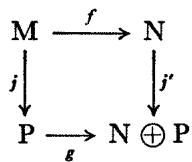
\includegraphics[keepaspectratio]{images/part004_a147f11a.jpg}}

where the vertical arrows are the canonical injections. Since g is injective and P is free, \(\bigwedge(g)\) is an injective homomorphism as has been seen above. Now, \(\bigwedge(j):\bigwedge(\mathbf{M})\to\bigwedge(\mathbf{P})\) is an injective homomorphism since M is a direct factor in P (no. 2). The composite homomorphism

\[
\bigwedge (\mathbf {M}) \xrightarrow {\bigwedge (j)} \bigwedge (\mathbf {P}) \xrightarrow {\bigwedge (g)} \bigwedge (\mathbf {N} \oplus \mathbf {P})
\]

is therefore injective and, as it is also equal to the composite homomorphism

\[
\Lambda (\mathbf {M}) \xrightarrow {\Lambda (f)} \Lambda (\mathbf {N}) \xrightarrow {\Lambda (j ^ {\prime})} \Lambda (\mathbf {N} \oplus \mathbf {P})
\]

we conclude that \(\bigwedge (f)\) is injective.

PROPOSITION 13. Let M be an A-module, N a direct factor submodule of M which is free of dimension p and \(\{u\}\) a basis of \(\bigwedge^{p}(\mathbf{N})\) . For an element \(x \in M\) to belong to N, it is necessary and sufficient that \(u \wedge x = 0\) .

Let P be a submodule of M complementary to N and let \(y \in N\) , \(z \in P\) be such that \(x = y + z\) . Then \(u \wedge x = u \wedge z\) . As \(\bigwedge^{p}(N)\) is free of dimension 1, the mapping \(\phi: P \to P \otimes \bigwedge^{p}(N)\) such that \(\phi(p) = p \otimes u\) is bijective (II, §3, no. 4, Proposition 4). On the other hand (no. 7, Proposition 10), the composition of the canonical homomorphisms

\[
\psi : \mathrm{P} \otimes \bigwedge^ {p} (\mathrm{N}) \rightarrow \bigwedge (\mathrm{P}) \otimes \bigwedge (\mathrm{N}) \rightarrow \bigwedge (\mathrm{M})
\]

is injective. The mapping \(\psi \circ \phi\) is therefore injective, whence the proposition.

THEOREM 2. Let \(\mathbf{M}\) be an A-module with a finite basis \((e_i)_{1\leqslant i\leqslant n}\) . For a sequence \((x_i)_{1\leqslant i\leqslant n}\) of \(n\) elements of \(\mathbf{M}\) to form a basis of \(\mathbf{M}\) , it is necessary and sufficient that the element \(\lambda \in \mathbf{A}\) such that

\[
x _ {1} \wedge x _ {2} \wedge \dots \wedge x _ {n} = \lambda . e _ {1} \wedge e _ {2} \wedge \dots \wedge e _ {n}\tag{23}
\]

be invertible in A.

Recall that \(e_{1} \wedge e_{2} \wedge \cdots \wedge e_{n}\) is the unique element of a basis of \(\bigwedge^{n}(\mathbf{M})\) (no. 8, Corollary 1 to Theorem 1) so that the element \(\lambda \in A\) satisfying (23) is determined uniquely. If \((x_{i})_{1 \leqslant i \leqslant n}\) is a basis of M, \(x_{1} \wedge x_{2} \wedge \cdots \wedge x_{n}\) is the unique element in a basis of \(\bigwedge^{n}(\mathbf{M})\) (no. 8), then \(\lambda\) is invertible. Conversely, suppose \(\lambda\) is invertible; then the alternating n-linear form f corresponding to the linear mapping \(g: \bigwedge^{n}(\mathbf{M}) \to \mathbf{A}\) such that

\[
g (e _ {1} \wedge e _ {2} \wedge \dots \wedge e _ {n}) = \lambda^ {- 1}
\]

is such that \(f(x_{1}, x_{2}, \ldots, x_{n}) = 1\) . For all \(x \in \mathbf{M}\) , obviously

\[
x \wedge x _ {1} \wedge \dots \wedge x _ {n} = 0
\]

(no. 3, Proposition 6); applying no. 8, Corollary 3 to Theorem 1, we obtain

\[
f (x _ {1}, x _ {2}, \dots , x _ {n}). x = \sum_ {i = 1} (- 1) ^ {i - 1} f (x, x _ {1}, \dots , \hat {x} _ {i}, \dots , x _ {n}). x _ {i}.
\]

As \(f(x_{1},\ldots ,x_{n}) = 1\) , this shows that every \(x\in \mathbf{M}\) is a linear combination of \(x_{1},x_{2},\ldots ,x_{n}\) and, as the latter are linearly independent (since

\[
x _ {1} \wedge x _ {2} \wedge \dots \wedge x _ {n} \neq 0),
\]

they form a basis of M.

